\documentclass[12pt]{article}
\usepackage[utf8]{inputenc}

%THIS IS WHERE ALL THE SYDE STUFF IS
\usepackage{sydestyle}

% Other imports go here
\usepackage{graphicx}
\graphicspath{{figures/}}
\usepackage{amsmath}


\title{Homework 1}
\classname{SYDE 543}
\author{Karan Thukral, 20460691, 4A}
\date{September 29, 2016}
\supervisortext{Course Instructor: Professor Shi Cao}

% Content here
\begin{document}

	% Start with a title page!
	\makereporttitle

	% Make a table of contents.
	\tableofcontents
	\newpage

	% Couldn't figure out how to automate this, but leave this line in to restart page numbers at 1 and with arabic numbers.
	\startarabicpagenumbers

	\section{Colour Blindness}
	The first example being examined is an application called "Trello". Trello is used in order to organize tasks across multiple people. This is done through the concepts of boards and heavily relies on colours to tag the tasks. Due to the heavy use of colour, the company has taken steps in order to imropve their usability for colour blind users. There is an option available that can be toggled to launch the app in a colour blind more. A side by side comparision is shown in Figure \ref{trelloimg}.
	
	\begin{figure}[!ht]
		\centering
		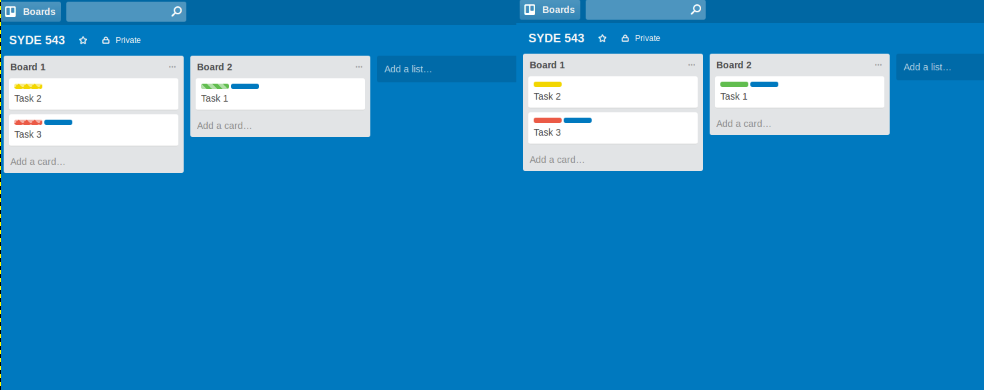
\includegraphics[width=1.0\textwidth]{trelloImage}
		\caption{Colour Blind Mode (Left) vs Regular Mode (Right)}
		\label{trelloimg}
	\end{figure}
	
	As it can be seen in Figure \ref{trelloimg} there are subtle differences in how the colours are displayed. Figure \ref{trelloLabels} shows the difference in more detail.
	
	\begin{figure}[!ht]
		\centering
		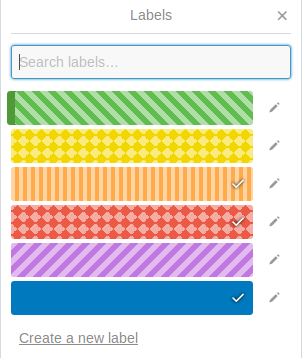
\includegraphics[width=0.2\textwidth]{trelloLabels}
		\caption{Colour Blind Mode Label Colours}
		\label{trelloLabels}
	\end{figure}
	
	As seen in the two figures during colour blind mode, Trello doesn't only rely on differentiation through colours. Instead Trello uses shapes and textures within the colour to differentiate between them. As an example, the only solid colour used is blue, where as for purple Trello has diagonal lines through it. Similarly unique patterns are used to make the colours/labels differentiable. Trello is an excellent example of using the knowledge (visual senses) from the cognitive ergonomics to make the product usable by a larger population. Due to the high reliance of the application on colours, without the colour blind more it would have been extreamly unusable for people suffering from colourblindness.
	
	\section{Sensory Adaption}
	This section will discuss the "Night Shift" feature on the iOS platform as an example for sensory adaption. Most displays act as an artifical source of lighting but also emit a significant amount of light in the spectrum of the blue wavelength. As per reaearch conducted blue wavelengths are useful during the day because they help boost attention, reaction time and mood. The same wavelegths of light at night are disruptive and can negatively affect sleep. In order to reduce or curb the negative effects of blue light, Apple added a new feature onto their iOS platform called "Night Shift". As the day continues, the phone screen changes the temperature of the light use and starts to use warmer tone after sundown. The aim behind this feature is to reduce the eye strain caused by a bright display especially at night (in darkness). The effect is shown in Figure \ref{nightshift}. This is a good example of the principle of adaption becuase it gives the user time to adjust to the change as its done gradualy throughout the day. I believe that this is good design and utilizes existing reaearch and cognitive ergonomics knowledge to provide the best user experience.
	
	\begin{figure}[!ht]
		\centering
		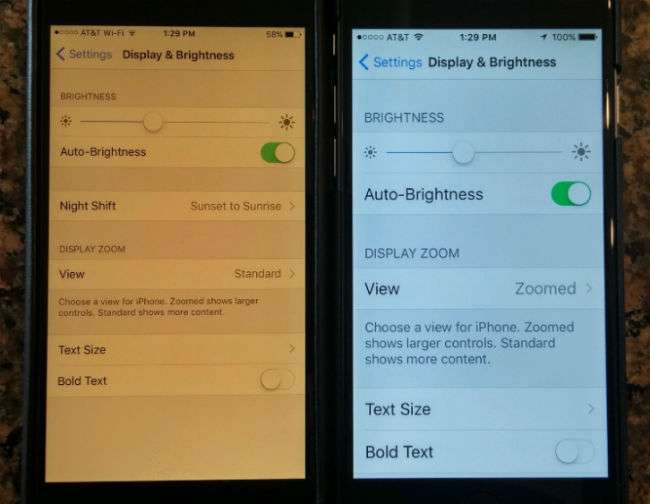
\includegraphics[width=0.5\textwidth]{nightshift}
		\caption{Night Shift On (Left) vs Off (Right)}
		\label{nightshift}
	\end{figure}
	
	\section{Haptic Feedback and Attention}
	The next example used is the Apple Watch and perticularly its map application. Due to the small screen of the watch, Apple had to use more than just the screen to convey information. As part of the map application Apple uses haptic feedback to alert the user of an upcoming turn. This is useful when walking or driving since it does not equire the user to look at the watch while trying to navigate. If the only source of information was text on the watch, the user would have to constantly keep checking it which can be dangerous while walking as it diverts the users attention from their environment and traffic. 
	
	Despite being useful, I personally feel that it can be improved. Since the watch only alerts the user that a turn is approaching and not which turn to make, it requires the user to check the watch everytime. This can lead to a lot of context switching for the user which deminishes the user experience. One way this can be imporved it by allowing the user to customize the haptic feedback pattern. This is already a feature available for call notifications on the iPhone. For example, for a left turn the watch can vibrate once and for right it can vibrate twice. This can be done in different ways by relying on length or intensity of the vibration or number of vibrations etc. Having this ability would make it possible for the user to reach their destination without having to look at the watch every time it vibrates.
	
	\section{Consistency}
	In order to discuss the principle of consistency, I am going to use the design of the Shopify admin. In order to look at an example of the principle in the admin, lets focus on the design of the butttons. Shopify does a really good job of having a small set of buttton designs which used through the admin. Once such example is every distructive button like "Delete Product" is coloured red (to signify danger) and such an action is always followed by a popup dialog to confirm the action. Two different occourances of this are shown in Figure \ref{delete-product} and \ref{delete-discount}. Similarly the delete button is always the right button on the dialogue and the "Cancel" button has a white background. Any action that does not affect state of the store has a white background and blue text. 
	
	\begin{figure}[!ht]
		\centering
		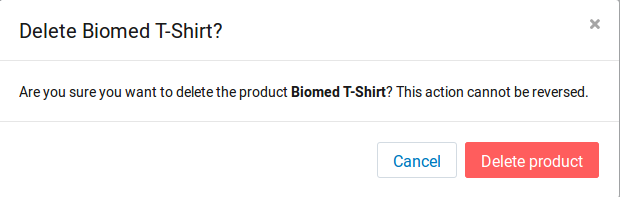
\includegraphics[width=0.5\textwidth]{delete-product}
		\caption{Delete Product Dialog}
		\label{delete-product}
	\end{figure}
	
	\begin{figure}[!ht]
		\centering
		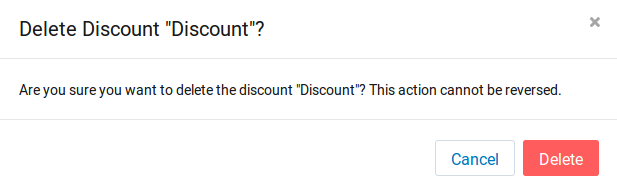
\includegraphics[width=0.5\textwidth]{delete-discount}
		\caption{Delete Discount Dialog}
		\label{delete-discount}
	\end{figure}
	
	The consistency throughout the admin reduces the congnivite workload for the user since the action type can be infered with only looking at the design and without having to read the text. One area where I feel like Shopify can improve is to use the red colour throughtout the admin. As an example, the "Delete Product" button the product page only becomes red when it is highlighted. Having it be a consistent red would inference extreamly easy.
	
	
\end{document}
